\documentclass{standalone}
\usepackage{tikz}
\usetikzlibrary{shapes,arrows.meta}
\begin{document}
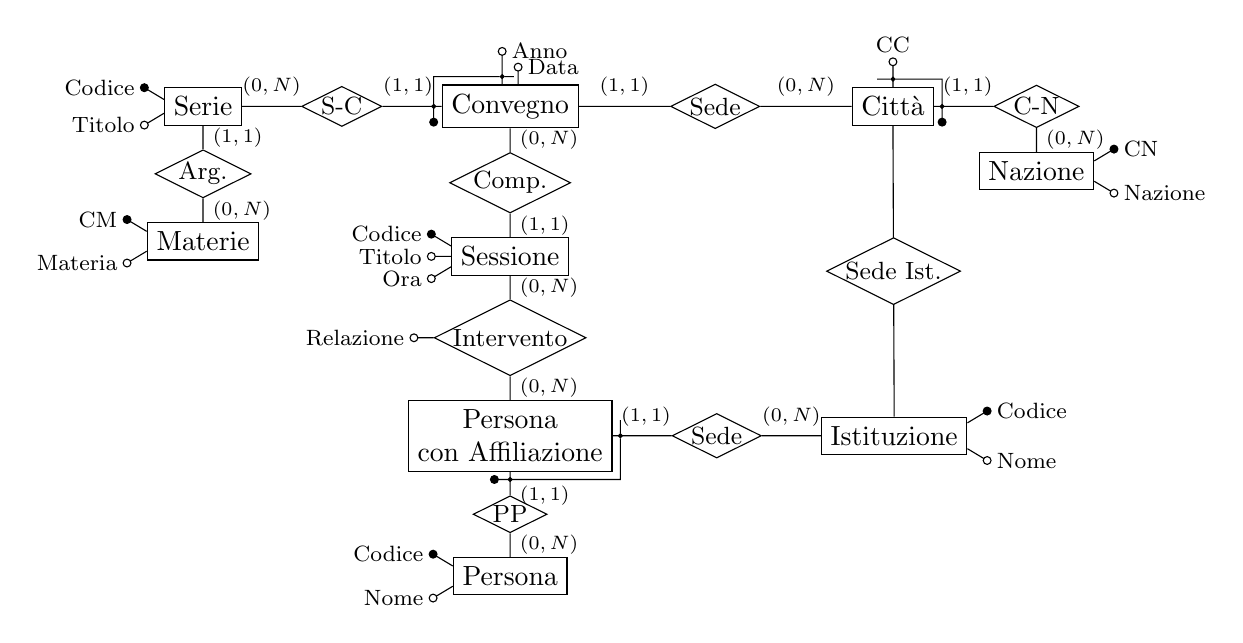
\begin{tikzpicture}
    \draw

    %%* Attributi:
    %%  node[draw, circle, inner sep=1pt, fill=black]{}node[right]{\footnotesize A}
    %%? Distanza orizzontale: E -(0.25,0.x)- A
    %%? Distanza verticale: E -(0,x * 0.22)- A

    %%* Cardinalità:a
    %%  node[below right]{\scriptsize $(0,N)$}
    %%  node[above right]{\scriptsize $(0,N)$}
    %%  node[midway, above]{\scriptsize $(0,N)$}

    %%* Relazione:
    %%  node[draw, diamond, shape aspect=2, inner sep=3pt, anchor=90](r1){}
    %%  node[draw, diamond, shape aspect=2, inner sep=0.2pt, anchor=180](r2){R2}

    %%* Entità:
    %%  node[draw, rectangle, anchor=90](e1){}
    %%? Distanza verticale: E -(0.3)- R -(0.3) E
    %%? Distanza orizzontale: E -(0.75)- R -(0.75)- E

    %%* Serie
    (0,0)node[draw, rectangle, anchor=90](serie){Serie}
    (serie.170)--++(-0.25,0.15) node[draw, circle, inner sep=1pt, fill=black]{}node[left]{\footnotesize Codice}
    (serie.190)--++(-0.25,-0.15)node[draw, circle, inner sep=1pt, fill=white]{}node[left]{\footnotesize Titolo}

    %%* Materie
    (serie.270)--++(0,-0.3)node[midway, right]{\scriptsize $(1,1)$}node[draw, diamond, shape aspect=2, inner sep=0.2pt, anchor=90](r1){\small Arg.}
    (r1.270)--++(0,-0.3)node[midway, right]{\scriptsize $(0,N)$}node[draw, rectangle, anchor=90](materie){Materie}
    (materie.170)--++(-0.25,0.15) node[draw, circle, inner sep=1pt, fill=black]{}node[left]{\footnotesize CM}
    (materie.190)--++(-0.25,-0.15)node[draw, circle, inner sep=1pt, fill=white]{}node[left]{\footnotesize Materia}

    %%* Convegno
    (serie.0)--++(0.75,0)node[midway, above]{\scriptsize $(0,N)$}node[draw, diamond, shape aspect=2, inner sep=0.3pt, anchor=180](r2){\small S-C}
    (r2.0)--++(0.65,0)node[draw, circle, inner sep=0.5pt, fill=black](a){}node[midway, above]{\scriptsize $(1,1)$}--++(0.1,0)node[draw, rectangle, anchor=180](convegno){Convegno}
    (convegno.110)--++(0,0.1) node[draw, circle, inner sep=0.5pt, fill=black](b){}--++(0,0.32)node[draw, circle, inner sep=1pt, fill=white]{}node[right]{\footnotesize Anno}
    (convegno.70) --++(0,0.22)node[draw, circle, inner sep=1pt, fill=white]{}node[right]{\footnotesize Data}
    (a)++(0,-0.2)node[draw, circle, inner sep=1pt, fill=black]{}|-(b)--++(0.15,0)
    

    %%* Città
    (convegno.0)--++(1.16,0)node[midway, above]{\scriptsize $(1,1)$}node[draw, diamond, shape aspect=2, inner sep=0.2pt, anchor=180](r3){\small Sede}
    (r3.0)--++(1.16,0)node[midway, above]{\scriptsize $(0,N)$}node[draw, rectangle, anchor=180](città){Città}
    (città.90)--++(0,0.1)node[draw, circle, inner sep=0.5pt, fill=black](b){}--++(0,0.22)node[draw, circle, inner sep=1pt, fill=white]{}node[above]{\footnotesize CC}

    %%* Nazione
    (città.0)--++(0.1,0)node[draw, circle, inner sep=0.5pt, fill=black](a){}--++(0.65,0)node[midway, above]{\scriptsize $(1,1)$}node[draw, diamond, shape aspect=2, inner sep=0.3pt, anchor=180](r4){\small C-N}
    (r4.270)--++(0,-0.3)node[midway, right]{\scriptsize $(0,N)$}node[draw, rectangle, anchor=90](nazione){Nazione}
    (nazione.10)--++(0.25,0.15)  node[draw, circle, inner sep=1pt, fill=black]{}node[right]{\footnotesize CN}
    (nazione.350)--++(.25,-0.15)node[draw, circle, inner sep=1pt, fill=white]{}node[right]{\footnotesize Nazione}
    (a)++(0,-0.2)node[draw, circle, inner sep=1pt, fill=black]{}|-(b)--++(-0.2,0)
    
    %%* Sessione 
    (convegno.270)--++(0,-0.3)node[midway, right]{\scriptsize $(0,N)$}node[draw, diamond, shape aspect=2, inner sep=0.2pt, anchor=90](r5){\small Comp.}
    (r5.270)--++(0,-0.3)node[midway, right]{\scriptsize $(1,1)$}node[draw, rectangle, anchor=90](sessione){Sessione}
    (sessione.170)--++(-0.25,0.15) node[draw, circle, inner sep=1pt, fill=black]{}node[left]{\footnotesize Codice}
    (sessione.180)--++(-0.25,0)    node[draw, circle, inner sep=1pt, fill=white]{}node[left]{\footnotesize Titolo}
    (sessione.190)--++(-0.25,-0.15)node[draw, circle, inner sep=1pt, fill=white]{}node[left]{\footnotesize Ora}

    %%* Persona con Affiliazione
    (sessione.270)--++(0,-0.3)node[midway, right]{\scriptsize $(0,N)$}node[draw, diamond, shape aspect=2, inner sep=0.2pt, anchor=90](r6){\small Intervento}
    (r6.270)--++(0,-0.3)node[midway, right]{\scriptsize $(0,N)$}node[draw, rectangle, anchor=90, align=center](pca){Persona\\con Affiliazione}
    (r6.180)--++(-0.25,0)node[draw, circle, inner sep=1pt, fill=white]{}node[left]{\footnotesize Relazione}


    %%* Persona
    (pca.270)--++(0,-0.1)node[draw, circle, inner sep=0.5pt, fill=black](a){}--++(0,-0.2)node[right]{\scriptsize $(1,1)$}node[draw, diamond, shape aspect=2, inner sep=0.3pt, anchor=90](r7){\small PP}
    (r7.270)--++(0,-0.3)node[midway, right]{\scriptsize $(0,N)$}node[draw, rectangle, anchor=90](persona){Persona}
    (persona.170)--++(-0.25,0.15) node[draw, circle, inner sep=1pt, fill=black]{}node[left]{\footnotesize Codice}
    (persona.190)--++(-0.25,-0.15)node[draw, circle, inner sep=1pt, fill=white]{}node[left]{\footnotesize Nome}
    
    %%* Istituzione
    (pca.0)--++(0.1,0)node[draw, circle, inner sep=0.5pt, fill=black](b){}--++(0.65,0)node[midway, above]{\scriptsize $(1,1)$}node[draw, diamond, shape aspect=2, inner sep=0.2pt, anchor=180](r8){\small Sede}
    (r8.0)--++(0.75,0)node[midway, above]{\scriptsize $(0,N)$}node[draw, rectangle, anchor=180](istituzione){Istituzione}
    (istituzione.90)--(città.270)node[midway, draw, diamond, shape aspect=2, inner sep=0.2pt, fill=white](r8){\small Sede Ist.}
    (istituzione.10)--++(0.25,0.15)  node[draw, circle, inner sep=1pt, fill=black]{}node[right]{\footnotesize Codice}
    (istituzione.350)--++(.25,-0.15)node[draw, circle, inner sep=1pt, fill=white]{}node[right]{\footnotesize Nome}
    (a)++(-0.2,0)node[draw, circle, inner sep=1pt, fill=black]{}-|(b)--++(0,0.2)
    

    ;
\end{tikzpicture}
\end{document}